%%%%%%%%%%%%%%%%%%%%%%%%%%%%%%%%%%%%%%%%%
% Masters/Doctoral Thesis 
% LaTeX Template
% Version 2.4 (22/11/16)
%
% This template has been downloaded from:
% http://www.LaTeXTemplates.com
%
% Version 2.x major modifications by:
% Vel (vel@latextemplates.com)
%
% This template is based on a template by:
% Steve Gunn (http://users.ecs.soton.ac.uk/srg/softwaretools/document/templates/)
% Sunil Patel (http://www.sunilpatel.co.uk/thesis-template/)
%
% Template license:
% CC BY-NC-SA 3.0 (http://creativecommons.org/licenses/by-nc-sa/3.0/)
%
%%%%%%%%%%%%%%%%%%%%%%%%%%%%%%%%%%%%%%%%%

%----------------------------------------------------------------------------------------
%	PACKAGES AND OTHER DOCUMENT CONFIGURATIONS
%----------------------------------------------------------------------------------------

\documentclass[
11pt, % The default document font size, options: 10pt, 11pt, 12pt
oneside, % Two side (alternating margins) for binding by default, uncomment to switch to one side
%catalan,
english,
%spanish,
singlespacing, % Single line spacing, alternatives: onehalfspacing or doublespacing
%draft, % Uncomment to enable draft mode (no pictures, no links, overfull hboxes indicated)
%nolistspacing, % If the document is onehalfspacing or doublespacing, uncomment this to set spacing in lists to single
%liststotoc, % Uncomment to add the list of figures/tables/etc to the table of contents
%toctotoc, % Uncomment to add the main table of contents to the table of contents
%parskip, % Uncomment to add space between paragraphs
%nohyperref, % Uncomment to not load the hyperref package
headsepline, % Uncomment to get a line under the header
%chapterinoneline, % Uncomment to place the chapter title next to the number on one line
%consistentlayout, % Uncomment to change the layout of the declaration, abstract and acknowledgements pages to match the default layout
]{MastersDoctoralThesis} % The class file specifying the document structure

\usepackage[utf8]{inputenc} % Required for inputting international characters
\usepackage[T1]{fontenc} % Output font encoding for international characters
\usepackage{eurosym}
\usepackage{footnote}
\usepackage{palatino} % Use the Palatino font by default
\usepackage{babel}
\usepackage[backend=bibtex,style=numeric,natbib=true,sorting=none]{biblatex}
\usepackage{multirow}
\usepackage{float}
\usepackage{tabularx}
\usepackage{listings}
\usepackage{xcolor}
\usepackage{appendix}
\usepackage{datetime}
\usepackage{array}
\usepackage{mathtools}
%\usepackage{fontspec}
%\setmainfont{Helvetica Neue Light}

\addbibresource{main.bib} % The filename of the bibliography

\usepackage[autostyle=true]{csquotes} % Required to generate language-dependent quotes in the bibliography

\newdate{date}{02}{03}{2018}
\date{\displaydate{date}}

%----------------------------------------------------------------------------------------
%	MARGIN SETTINGS
%----------------------------------------------------------------------------------------

\geometry{
	paper=a4paper, % Change to letterpaper for US letter
	inner=2.5cm, % Inner margin
	outer=3cm, % Outer margin
	bindingoffset=.5cm, % Binding offset
	top=1.5cm, % Top margin
	bottom=1.5cm, % Bottom margin
	%showframe, % Uncomment to show how the type block is set on the page
}

%----------------------------------------------------------------------------------------
%	THESIS INFORMATION
%----------------------------------------------------------------------------------------

\thesistitle{Skyscanner offer and demand comparison} % Your thesis title, this is used in the title and abstract, print it elsewhere with \ttitle
\supervisor{Javier Arias} % Your supervisor's name, this is used in the title page, print it elsewhere with \supname
\examiner{} % Your examiner's name, this is not currently used anywhere in the template, print it elsewhere with \examname
\degree{Computer Engineering Degree} % Your degree name, this is used in the title page and abstract, print it elsewhere with \degreename
\author{Fèlix Arribas} % Your name, this is used in the title page and abstract, print it elsewhere with \authorname
\addresses{} % Your address, this is not currently used anywhere in the template, print it elsewhere with \addressname

\def \universitysupervisor{Maria José Casañ}

\keywords{} % Keywords for your thesis, this is not currently used anywhere in the template, print it elsewhere with \keywordnames
\university{Universitat Politècnica de Catalunya (UPC)} % Your university's name and URL, this is used in the title page and abstract, print it elsewhere with \univname
\department{\href{https://www.essi.upc.edu/}{Software Engineering and Information Systems department}} % Your department's name and URL, this is used in the title page and abstract, print it elsewhere with \deptname
\group{\href{https://www.essi.upc.edu/}{ESSI}} % Your research group's name and URL, this is used in the title page, print it elsewhere with \groupname
\faculty{\href{http://www.fib.upc.edu}{Facultat d'Informàtica de Barcelona (FIB)}} % Your faculty's name and URL, this is used in the title page and abstract, print it elsewhere with \facname

\def \company{Skyscanner}
\def \tribe{Marketplace Engine tribe}
\def \squad{DeLorean squad}

\AtBeginDocument{
\hypersetup{pdftitle=\ttitle} % Set the PDF's title to your title
\hypersetup{pdfauthor=\authorname} % Set the PDF's author to your name
\hypersetup{pdfkeywords=\keywordnames} % Set the PDF's keywords to your keywords
\hypersetup{linkcolor=black}
}

\newcolumntype{L}{>{\centering}m{0.75cm}}
\newcolumntype{M}{m{9cm}}
\newcolumntype{T}{m{12cm}}

\newcommand\tab[1][0.75cm]{\hspace*{#1}}


\colorlet{punct}{red!60!black}
\definecolor{background}{HTML}{EEEEEE}
\definecolor{delim}{RGB}{20,105,176}
\colorlet{numb}{magenta!60!black}

\lstdefinelanguage{json}{
    basicstyle=\normalfont\ttfamily,
    numbers=left,
    numberstyle=\scriptsize,
    stepnumber=1,
    numbersep=8pt,
    showstringspaces=false,
    breaklines=true,
    frame=lines,
    backgroundcolor=\color{background}
}

\lstdefinelanguage{java}{
    basicstyle=\normalfont\ttfamily,
    numbers=left,
    numberstyle=\scriptsize,
    stepnumber=1,
    numbersep=8pt,
    showstringspaces=false,
    breaklines=true,
    frame=lines,
    backgroundcolor=\color{background}
}

\setlength{\parindent}{0pt}

\begin{document}
\selectlanguage{english}

\frontmatter % Use roman page numbering style (i, ii, iii, iv...) for the pre-content pages

\pagestyle{plain} % Default to the plain heading style until the thesis style is called for the body content

%----------------------------------------------------------------------------------------
%	TITLE
%----------------------------------------------------------------------------------------

\begin{titlepage}
\begin{center}


\includegraphics[scale=0.25]{resources/logo-skyscanner.png}


\includegraphics[scale=0.1]{resources/logo-upc.png} % University/department logo - uncomment to place it

\vspace*{.04\textheight}
{\scshape\LARGE \href{https://www.skyscanner.net/}{\company}\\ in collaboration with\\ \href{http://www.upc.edu}\univname\par}\vspace{1.5cm} % University name
\textsc{\Large Final Degree Project}\\[0.5cm] % Thesis type

\HRule \\[0.4cm] % Horizontal line
{\Huge \bfseries \ttitle\par}\vspace{0.4cm} % Thesis 
{\large Skyscanner's data comparison\par}\vspace{0.1cm} % Thesis title
\HRule \\[1.5cm] % Horizontal line
 
\begin{minipage}[t]{0.4\textwidth}
\begin{flushleft} \large
\emph{Author:}\\
\authorname % Author name - remove the \href bracket to remove the link
\end{flushleft}
\end{minipage}
\begin{minipage}[t]{0.4\textwidth}
\begin{flushright} \large
\emph{Director:} \\
\supname % Supervisor name - remove the \href bracket to remove the link  
\\
\emph{University supervisor:} \\
\universitysupervisor
\end{flushright}
\end{minipage}\\[3cm]
 
\vfill

\large \textit{A Project for the}
\large \degreename 
\textit{ in the}\\[0.2cm]
\deptname\\[0.2cm]
\facname\\[0.2cm]
\textit{working with}\\[0.2cm]
\squad
\textit{ from}
\tribe\\
\vfill

{\large \displaydate{date}}\\[4cm] % Date
 
\vfill
\end{center}
\end{titlepage}

%----------------------------------------------------------------------------------------
%	ABSTRACT
%----------------------------------------------------------------------------------------

\begin{abstract}
\addchaptertocentry{\abstractname}
In the last century, the world has became smaller. Communications are easier and faster than fifty years ago. Back then, you could talk through a fix phone, but you were not able to send any kind of media, like photos, videos, etc. Only the latest technology of that moment was able to do that. Since the smart phone revolution in 2007 almost everyone can text messages, sending images, share live videos or almost whatever you can imagine in less than a second.
\\\\
But the internet, phones and communications are not the only thing that made the world smaller. Ways of traveling helped to this earth flattering too. In 1918 visiting another place was very difficult. If you wanted to go through the sea, you had to do it by boat. The fastest way to travel very far in a continent was by train, but not all places were connected with rails. Nowadays, all along with the internet revolution, anyone can travel to the other side of the world in less than a day by plane. Even for traveling inside the same country people use planes.
\\\\
But, is the air industry as efficient enough? Are all airlines users satisfied with their purchases and possibilities? \company\ provides an easy to use tool to search cheap flights from any airport to another. Sadly, sometimes is difficult for users to find what they really want.
\\\\
This project wants to help solving this problem, providing a HeatMap to explore differences and similarities between what users search and what airlines provides. Being able to compare between specific dates to guess user behavior.
\end{abstract}

%----------------------------------------------------------------------------------------
%	TABLE OF CONTENTS
%----------------------------------------------------------------------------------------

\tableofcontents

%----------------------------------------------------------------------------------------
%   THESIS CONTENT - APPENDICES
%----------------------------------------------------------------------------------------

\mainmatter

\pagestyle{thesis}

% Chapter 1: Context

\chapter{Context}

\label{chapter01}

This is a project developed in \textit{\company} and evaluated by the \textit{\univname} as a Final Degree Project.
\\\\
This project's purpose is to compare \textbf{user demand} and \textbf{flights provided} by airlines for routes. This comparison could improve flights advertisement according to user demand. The company could also develop complex software using the huge amount of data it will compare through an Application Programming Interface.
\\\\
\company\ have more than 75 million flights information and about 13 million users queries every day. In order to compare all the data available and get significant results, the software should solve  \textbf{Big Data}.

%-----------------
%   SECTION 1.1
%-----------------

\section{\company}

\company\cite{skyscanner_strategy} is a travel fare aggregate website. It was formed in 2004 when a group of people was frustrated by the difficulties of finding cheap flights.
\\\\
In 12 years has evolved from a little office in the suburbs of Edinburgh to a world wide company with ten offices in seven different countries. In the next 5 years, \company\ wants to become the travel experience that people prefer to the myriad confusing and unconnected travel apps.
\\\\
Now, is one of the top travel fare aggregate website. It has more than 4 million visitors every day and, more or less, a revenue of half a million pounds per day.
\\\\
Before joining \company\ I wondered how they growth that fast and how they did this amount of money. Usually, \textit{if you do not pay for the product, you are the product}, so my first thoughts were that \company\ sell user searches, and travel tendencies to airline companies. \textbf{Companies know what travelers buy, but now what they have searched before their final purchase.}
\\\\
Once inside the company, I realized that it is not the way \company\ make money. Knowing that, when I joined \squad\ in Barcelona and had the opportunity to make the final degree project there, I proposed a tool to get traveler tendencies and compare them to \squad's data, timetables and flights.

%-----------------
%   SECTION 1.2
%-----------------

\section{\squad}

DeLorean\cite{delorean_squad_home} is a squad of \tribe\footnote{Learn more about \textit{\nameref{appendix_a}} in Appendix A}, its mission is to provide the best data and services around the routes, timetables and modes of transportation to go from one point on Earth to another.

%-----------------
%   SECTION 1.2
%-----------------

\section{\tribe}

This tribe\cite{marketplace_engine_home} is one of the most important tribes in \company, its mission is to provide the most comprehensive and accurate flight inventory for \company\ and her partners with minimum latency.
\\\\
Its main goal is to evolve the search, pricing, routes and browse services to be horizontally scalable and set us up to build a lightning fast, super accurate and fully comprehensive flight search engine, enabling the traveler to instantly find the best flight at the best price with minimum effort.


% Chapter 2: State-of-the-art

\chapter{State-of-the-art}

\label{chapter02}

Since this project is not oriented for \company\ users but the company itself, the \textit{\nameref{chapter02}} relates to services inside \company. Even so, a brief explanation about other metasearch engines would help to find the gap this project is developed.

%-----------------
%   SECTION 2.1
%-----------------

\section{Fare aggregators and metasearch engines}

\subsection{Google Flights}

In the last years Google Flights has became the main competitor of \company. The new version is very fast and has a complete new interface, following Android guidelines.
\\\\
Google is one of the top tech companies worldwide and has a lot of different platforms. It is a competitor to be aware of, the integration with Gmail, Google Calendar and Android OS makes Google Flight a part of Google's ecosystem. The traveler may feel comfortable.

\subsection{Kayak}

Kayak has always been the main competitor, both companies started in 2004. Unlike \company, Kayak started with Flights, Hotels and Car hiring. \company\ added those two extra search engines between 2013 and 2014.

\subsection{Expedia}

Launched in November 1998, is one of the oldest fare aggregator and metasearch engine. Apart of its own website, is also a \company\ provider. Some of the prices are taken from Expedia and sometimes the user is redirected to their website to finish their purchase.

%-----------------
%   SECTION 2.2
%-----------------

\section{\company\ services}

In \company\ the user has never been a product, in fact, one of the statements of \company's culture says \textit{Traveler != Product}\cite{the_road_ahead}.
\\\\
There has never been a project getting value from user information because it does not follows the company culture, so the definition of the problem and the scope of the project must be very accurate to ensure it is fulfilling with \company's strategy\cite{skyscanner_strategy}.

\subsection{Marketplace Engine} \label{mp_engine}

This tribe is formed by five squads, those constantly work to improve the routes and pricing service all along with an efficient search.
\\\\
Marketplace Engine works with data \textit{from the provider to the user}. In other words, it just serves \textbf{information to the user} but does not get any from him/her. All five squads take all the \textbf{data from providers}.

\begin{figure}[H]
\centering
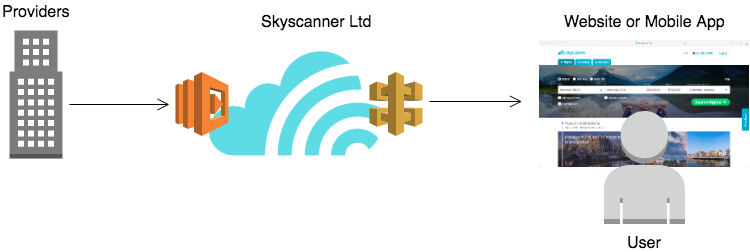
\includegraphics[scale=0.45]{diagrams/state-of-the-art-tribes-mp.png}
\caption{Simple explanation of Marketplace Engine data flow.}
\end{figure}

\subsection{Data Tribe} \label{data_tribe}

In the other hand, Data Tribe has a lot of squads with services used to collect \textbf{data from user's activity}. The flow of the information is \textit{from the user to \company}.

\begin{figure}[H]
\centering
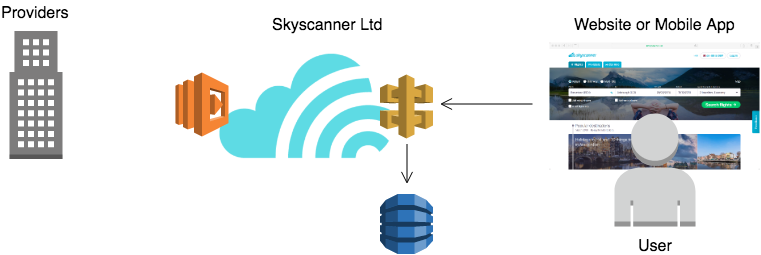
\includegraphics[scale=0.45]{diagrams/state-of-the-art-tribes-data.png}
\caption{Simple explanation of Data Tribe data flow.}
\end{figure}

\subsection{The gap}

There is no tribe or squad that works with both \textbf{data sources}: Providers and Users. And here is where the \textit{Heatmap} will be.

\begin{figure}[H]
\centering
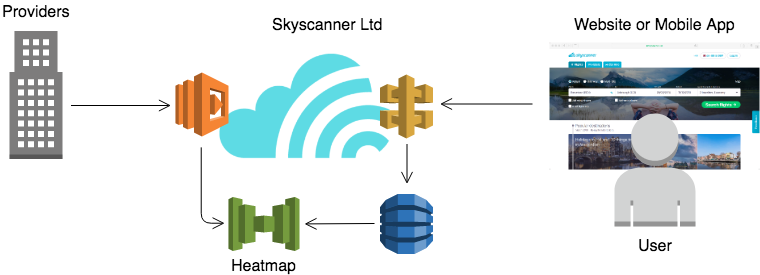
\includegraphics[scale=0.45]{diagrams/state-of-the-art-tribes-hm.png}
\caption{First approach of the Heatmap's data flow.}
\end{figure}


% Chapter 3: Scope of the project

\chapter{\company\ Heatmap}

\label{chapter03}

%-----------------
%   SECTION 3.1
%-----------------

\section{Formulation of the problem} \label{problem}

The main goal of this project is creating a tool for \textit{\company} to ease the routes and airports comparison by different parameters, taking into account values like \textbf{user demand} and \textbf{flights provided} by airlines.
\\\\
In any team of \company, user queries and providers data is compared in order to guess valuable trends.
\\\\
Found that gap, a bunch of new ideas appeared. After some talks with product owners of different squads and some senior engineers, a promising idea showed up:
\\\\
Comparison of \textbf{user demand} and \textbf{flights offered} by airlines, enabling finding \textit{over-requested} routes or airports. Those routes or airports with more user demand than offers by the providers.
\\\\
\squad\ manages a huge amount of data: All flights planned for the next two years, this are more than 75 million records. The database of all user queries in the website or mobile application is even bigger\footnote{For instance, if there were only one query per visitor the database would have 4 million new records per day}. Not much more information needed to say that this is \textbf{Big Data} problem.
\\\\
With \squad's product owner help, we found some use cases for the processing of those 75 million routes and all user session's queries to get some significant results:
\\\\
Provide a \textbf{visual tool} to find routes and airports with much \textbf{more demand than offer} and be able to observe the \textbf{evolution} of it {through time}:

\begin{itemize}
  \item A route or airport with a lot of demand, but not enough offer to cover it, will be \textbf{over-requested}.
  \item A route or airport with much more offer, but not that amount of demand, will be \textbf{non-profitable}.
\end{itemize}

%-----------------
%   SECTION 3.2
%-----------------

\section{Scope}

Merging both data sources (providers and users) generates a lot of new valuable data with a lot of different application: From simply selling it to providers, to complex deep learning systems.
\\
The final goal of this project is displaying the comparison in a simple Web UI for Marketing squads or tribes. This can be split in three smaller goals or components:

\subsection{Pipeline}

Distributed application that maps and merge all the data from both sources in its given format to the required data model.
\\\\
The pipeline reads from \nameref{mp_engine} and \nameref{data_tribe} services. Then, it maps the provider and user data to the desired data model. The new entities are stored in a database where the service will read from.
\\\\
The application will be split in two sub applications, one for providers data and other for users. So both of them can vary independently without depending on each others' sources and changes may have in the future.

\subsection{Service}

Simple HTTP Service with a basic Application Programming Interface to serve Pipeline's results. The service will have an internal endpoint only available for other \company\ applications or developers.

\subsection{Visual representation} \label{visual_representation}

Website with a visual representation of the data. There are plenty of ways to draw charts and maps visualizations. The Web UI will be composed by three main pages:

\subsubsection*{World Map}

Interactive world map with all airports represented with a dot. The radius of the dot depends on the amount of flights the airport operates.
\\\\
The Heatmap user will be able to select an airport, set a date and go to \nameref{chart_visualization} page. Another option is to select two airports, first the origin, then the destination, set a date and go to the \nameref{chart_visualization} page. If the user does not want to select the entity through the map, he/she can search it using the \nameref{browser}.

\begin{figure}[H]
\centering
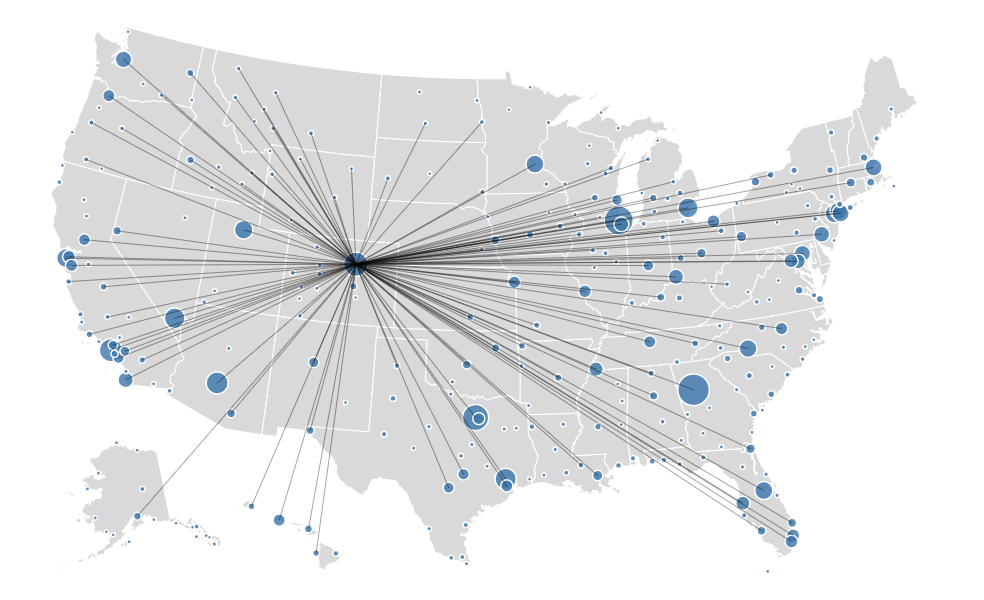
\includegraphics[scale=0.2]{resources/us-map-example01.png}
\caption{Example of the world map style. Only displaying the US to make it look clearer.}
\end{figure}

\subsubsection*{Browser} \label{browser}

Simple browser with two tabs: \textit{Route} and \textit{Airport}. In the route browser will appear three input text fields, one for the origin airport, the second for the destination and the last one for the date. In the airport browser will only appear two input text fields, airport and date.
\\\\
Once the inputs are set, the user will be able to click the \textit{Search} button and move to the next page.

\subsubsection*{Chart visualization} \label{chart_visualization}

Simple chart with the comparison between providers offer and user demand of the selected entity through time.

\begin{figure}[H]
\centering
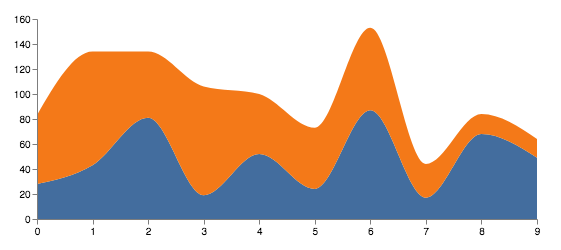
\includegraphics[scale=0.4]{resources/stacked-chart-example01.png}
\caption{Chart mock-up. One color goes for Providers Offer and the other one for User Demand.}
\end{figure}

\subsection{Not list} \label{not_list}

It is also important to define what this project will \textbf{not} be.

% WIP
\begin{itemize}
  \item \textbf{Prices} or \textbf{quotes}: In any moment will check for flight prices or quotes.
  \item \textbf{Carriers}, \textbf{cities} and \textbf{countries}: The comparison will be only available between routes and airports, not airlines (carriers), cities nor countries.
  \item \textbf{Create}, \textbf{update} or \textbf{delete} data through the \textbf{Server}: The only input will come from the pipeline. Entities are never deleted or modified in order to keep historical data.
  \item \textbf{Create}, \textbf{update} or \textbf{delete} data through the \textbf{Web UI}: The only input will come from the pipeline. Entities are never deleted or modified in order to keep historical data.
\end{itemize}

%-----------------
%   SECTION 3.3
%-----------------

\section{Risks}

There are several risks can appear while developing the project. Most risks appear because of the dependencies with other tribes and squads and dependencies with other services. In the other hand, all performance risks of the Pipeline can be ignored because \company's hardware is enough for big applications, like this one.

\subsection{Routes contract}

\squad's routes service is under development and during the Heatmap development the routes data model may change a little bit. For example, the origin and destination recently changed: In December 2017 the service was giving an \textit{Airport ID}, but now is giving an Airport object with more parameters like IATA Code\cite{iata_code}, Country ID, City ID, etc.

\subsection{Users information}

In the website and mobile application, the user have plenty of different ways to search the perfect flight. The most common one is by origin, destination and date, but he/she can also search by month or by destination. The user does not search flights for a given route in a given date. It sets the period of time he/she can travel and \company\ offers cheap destinations.
\\\\
This way of searching flights may be difficult for comparing with routes and airports offer, because sometimes the route is the actual result and not the query.

\subsection{Amount of data}

As explained before in the \nameref{problem}, there is a very big amount of data that need to be mapped. Luckily, \company\ have great cloud machines and \textit{unlimited} space\footnote{Read more in section \nameref{res_and_env}}. Anyway, still an issue to be aware of.

\subsection{Web UI}

Creating the interactive map and plots for the proposed website from zero, is a whole project itself. In order to avoid failing in the \textit{\nameref{visual_representation}} goal, the best option is to use reliable libraries, like Vega\cite{vega}.

%-----------------
%   SECTION 3.4
%-----------------

\section{Methodology and rigor} \label{methodology_rigor}

\subsection{Extreme Programming} \label{xp}

This project will be developed along with \squad's work. This squad is following Scrum, an agile methodology. After some research and discussions with the rest of the team, Extreme Programming (XP)\cite{xp} showed up as the best option.
\\\\
XP is a style of software development focused in excellent applications, programming techniques and clear communication. To accomplish that, XP includes a philosophy of software development, body of practices, complementary principles and a community that shares these values.
\\\\
This methodology works with short development cycles, resulting in early, concrete and continuing feedback. Has an incremental approach, making way to a flexible schedule for the implementation. It relies in oral communication and tests to reach the goal of the project.
\\\\
The original Extreme Programming methodology is for teams of developers, but this project will be only developed by myself, so the original idea has been modified a little bit. The pair programming and pair negotiation has been removed because I have nobody to pair with. In order to have some feedback and update the requirements properly with the supervisor, Francisco López, approval, I will be attending all \squad\ stand up meetings and explaining my progress and, if necessary, create meetings with the product owner and the rest of the squad to take the project on the right track.

\begin{figure}[H]
\centering
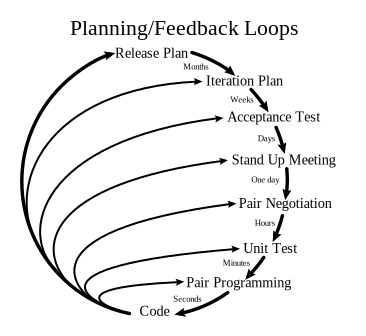
\includegraphics[scale=0.25]{diagrams/extreme_programming.png}
\caption{Extreme programming planning loops.}
\end{figure}

\subsection{GitLab}

This platform will be the main tool for version control of the source code and issue tracking of different tasks.

\subsubsection*{\texttt{git}}

All code projects (pipelines, service and website) will be stored in my personal projects space in \company's GitLab domain. Task and issue projects will be related to each project.
\\\\
Using \texttt{git}, the versions will be forked in branches, each branch will stand for an specific issue. \textit{Master} will be the main branch where the latest production version will be.

\subsubsection*{Tasks and issues}

The \textbf{issue tracking} will be very helpful in order to monitor the evolution of the project. Issues will be composed by a title, description, milestone, labels (if needed), due date and weight, and represents a new functionality. In order to know the status, issues will be listed in three columns:
\\\\
\textbf{Backlog:} Known tasks that haven been started yet. Could be a well defined task, with a very clear description, a due date and weight, or just a draft with empty fields.
\\
\textbf{WIP:} Work in Progress. The task is being considered, developed or tested.
\\
\textbf{Done:} Tasks finished, tested and working fine. Ready for production.

% Chapter 4: Requirements analysis

\chapter{Requirements analysis}

\label{chapter04}

\section{Actors}

Initially it seemed difficult to find stakeholders and actors in these project apart from the providers. It is not a tool for the user of \company\, so, as explained before, one risk of these project was not finding enough support.
\\\\
After walking with the Squad Lead and then the Product Own of \squad\ a lot of stakeholders appeared: DeLorean Squad, Marketing Automation Squad, State Machine Squad, etc. Each of these stakeholders has different use cases and the project became very interesting for a considerable part of \company\ .

\subsection{DeLorean Squad}

The mission of \squad\ is to provide the best data and services around the routes, timetables and modes of transportation to go from one point on Earth to another.
\\\\
Right now, \squad\ provides a very fast service that serves flights logistic information between a given origin and destination. Some information you can find in a route is the fight number, carriers, stops, date ranges, etc. These flights are just \textbf{single ticket flights}. The squad is currently working on more complex routes, constructed routes\footnote{Contructed Timetable contains constructed routes, routes composed by two or more single ticket flights.}.
\\\\
The constructed routes timetable is under construction, so is not available for these project. The Heatmap relies on the timetable of Single Flight Number service, also known as Timetable SFN Service.

\subsubsection{Timetable SFN Service}

The \textit{timetable SFN} endpoint returns details for time tabled Single Flight Number itineraries series. Note that SFNs are not ticket-able, so they do not include itineraries which cannot be bought on their own, neither the price nor restrictions.
\\\\
Timetable SFN Service provides all the \textbf{current} flights. This is a little bit of a problem when trying to get past routes: Timetable SFN Service does not provide past flights information, it is always \textbf{up-to-date}. In order to get this data it is needed to go one step back in the whole DeLorean data processing: Timetable Ingest Pipeline.
\\\\
Tech specifications of Timetable SFN Services are explined in section %\ref{$LABEL}.

\subsubsection{Timetable Ingest}

This phase, basically collects all the OAG\footnote{OAG file (also know as WTF file), is a CSV\cite{csv} file which each row represents a timetable for a Single Flight Number.} from a provider and maps it into routes in JSON\cite{json} format. For each different version of the OAG file, the pipeline creates a new file with all the routes.
\\\\
Then, in order to get past routes, the heatmap reference in old versions of the file created by the Timetable Ingest Pipeline.
\\\\
Tech specifications of Timetable Ingest Pipeline are explined in section %\ref{$LABEL}.

\subsection{Product Owner} \label{product_owner}

\textbf{Jen Agerton} is the Product Owner of DeLorean Squad, 

\subsection{DeLorean's Squad Lead}

\textbf{Francisco López}, who is also the supervisor of this project, and I has the initial idea for this project. He oriented it for a Machine Learning purpose.

\subsection{Neil Ross}

Neil Ross is currently the Squad Lead of \ref{marketing_atomation_squad}, this contact was given to me from my \ref{product_owner} Jen Agerton.
\\\\
After some talks through Slack\cite{slack}, he forward me extracts of the email he sent when he was in RaTS Squad, regarding to their use cases. Most of the use cases have been used for this project.

\subsubsection{Fuel RaTS Squad}

Routes and Timetable Servies Squad provides the best data and services around the routes, timetables and modes of transportation to go from one point on Earth to another. Fuel RaTS has the same mission as DeLorean Squad, but develop different services. Since Fuel RaTS provides basic routes data, pricing, live update information and multi-destination combinationcs, \squad\ provides a very fast service for only routes.

\subsubsection{Marketing Automation squad} \label{marketing_atomation_squad}

Marketing Automation squad enables scalable growth by automating workflows, and the collection of insightful data. They have three main goals:

\begin{itemize}
  \item Provide data to support decision making
  \item Automated, data driven campaign management
  \item Budget process automation
\end{itemize}

MAS provides fourteen 

\subsection{Providers}

\subsection{Competitors}

\section{Functional requirements}

\section{Non functional requirements}

\section{Use cases}

% ...
% Chapter 5: Project planning

\chapter{Project planning}

\label{chapter05}

Before defining tasks and time distribution of those, it is important to remember that this project will be developed under an Agile Methodology, \nameref{xp}. XP attempts to reduce costs of changes in requirements and long term plans, this means that this \textit{time planning} will provably change during the development. Every week a small iteration plan will be made in order to adjust the tasks with the scope and time of the project.
\\\\
Even so, here is a general plan. Tasks has been \textbf{grouped regardless the technology}, for instance: Task 27, Home Page from the Web UI. It will be developed in HyperText Markup Language and Java Script, but there is only one task for it. As explained in the previous paragraph, it is defined this way for now, in order to be agile in changes of the requirements. Then, tasks are grouped in \textbf{Milestones}.
\\\\
Milestones are used to mark specific points or goals along of a project \textit{timeline}. Milestones are very useful in order to do not losing time perception in long software projects when using Agile Methodologies, in which there are not usually to many deadlines.
\\\\
Another important thing to take into account is the \textbf{tasks overlapping}. Is a good practice\cite{clean_coder} not to work to much time in the same thing, task or goal. Swapping between different tasks and milestones can help so the developer \textbf{does not obfuscate}.
\\\\
Last but not least, there are two holiday weeks in March, one is \textit{Holy week} (13th), and the other is extra. That is why the project starts earlier.

%-----------------
%   SECTION 5.1
%-----------------

\section{Tasks}

Development tasks (from 14 to 30) duration is specified in days. Weeks are composed by five working days, so 5 days equals to a week. In a day, the developer is supposed to work five hours. From week seven to week twenty-three, there are fifteen working weeks (not counting holidays). Doing simple maths, the development will take:
\\
$$15\ \textrm{weeks} \times 5\ \frac{\textrm{days}}{\textrm{week}} \times 5\ \frac{\textrm{hours}}{\textrm{day}} = 375\ \textrm{hours}$$
\\
\textbf{375 hours} of development.
\\\\
It is important to understand that similar tasks like 16th and 20th or 17th and 21st have different times, that is because the second time it is supposed to be very similar than the first, so there will be some previous knowledge when executing it for second time.

%-------------------
%   SECTION 5.1.1
%-------------------

\subsection{Inception}

Regard this an agile project, there has been an small inception part where the project was predefined and explained to \company\ product owners to see if it was viable.

\begin{table}[H]
\begin{tabular}{>{\raggedleft\arraybackslash}p{3cm}>{\raggedright\arraybackslash}p{11cm}}
\textbf{Name}        & Inception \\
\textbf{Number}      & 1 \\
\textbf{Description} & Identify the initial scope of the project, stakeholders, context and environment where the project will be developed. \\
\textbf{End date}    & 9th of February, 2018 \\
\end{tabular}
\label{milestone1}
\end{table}

\begin{table}[H]
\begin{tabular}{>{\raggedleft\arraybackslash}p{3cm}>{\raggedright\arraybackslash}p{11cm}}
\textbf{Name}        & Definition of the problem \\
\textbf{Number}      & 2 \\
\textbf{Description} & Defining, at a high level, what the system will do. \\
\textbf{Duration}    & 10 days \\
\textbf{Milestone}   & \nameref{milestone1} \\
\textbf{Dependencies}& -- \\
\end{tabular}
\end{table}

\begin{table}[H]
\begin{tabular}{>{\raggedleft\arraybackslash}p{3cm}>{\raggedright\arraybackslash}p{11cm}}
\textbf{Name}        & Scope \\
\textbf{Number}      & 3 \\
\textbf{Description} & What the software project will do and will not. Not list. \\
\textbf{Duration}    & 5 days \\
\textbf{Milestone}   & \nameref{milestone1} \\
\textbf{Dependencies}& 2: Definition of the problem \\
\end{tabular}
\end{table}

\begin{table}[H]
\begin{tabular}{>{\raggedleft\arraybackslash}p{3cm}>{\raggedright\arraybackslash}p{11cm}}
\textbf{Name}        & Risks \\
\textbf{Number}      & 4 \\
\textbf{Description} & Find possible problems and obstacles may appear in the future development. \\
\textbf{Duration}    & 8 days \\
\textbf{Milestone}   & \nameref{milestone1} \\
\textbf{Dependencies}& 3: Scope \\
\end{tabular}
\end{table}

\begin{table}[H]
\begin{tabular}{>{\raggedleft\arraybackslash}p{3cm}>{\raggedright\arraybackslash}p{11cm}}
\textbf{Name}        & Scope refinement \\
\textbf{Number}      & 5 \\
\textbf{Description} & After finding the risks, review the scope. Make it possible. \\
\textbf{Duration}    & 4 days \\
\textbf{Milestone}   & \nameref{milestone1} \\
\textbf{Dependencies}& 4: Risks \\
\end{tabular}
\end{table}

\begin{table}[H]
\begin{tabular}{>{\raggedleft\arraybackslash}p{3cm}>{\raggedright\arraybackslash}p{11cm}}
\textbf{Name}        & Environment \\
\textbf{Number}      & 6 \\
\textbf{Description} & Find the correct environment in order to build the project. \\
\textbf{Duration}    & 2 days \\
\textbf{Milestone}   & \nameref{milestone1} \\
\textbf{Dependencies}& 5: Scope refinement \\
\end{tabular}
\end{table}

%-------------------
%   SECTION 5.1.2
%-------------------

\subsection{Project management}

\begin{table}[H]
\begin{tabular}{>{\raggedleft\arraybackslash}p{3cm}>{\raggedright\arraybackslash}p{11cm}}
\textbf{Name}        & Project management (GEP) \\
\textbf{Number}      & 7 \\
\textbf{Description} & First stage in the TFG. Get thesis started. \\
\textbf{End date}    & 20th of April, 2018 \\
\end{tabular}
\label{milestone2}
\end{table}

\begin{table}[H]
\begin{tabular}{>{\raggedleft\arraybackslash}p{3cm}>{\raggedright\arraybackslash}p{11cm}}
\textbf{Name}        & Context and scope \\
\textbf{Number}      & 8 \\
\textbf{Description} & Indicate general objective of the TFG and context. \\
\textbf{Duration}    & 12 days \\
\textbf{Milestone}   & \nameref{milestone2} \\
\textbf{Dependencies}& -- \\
\end{tabular}
\label{deliverable1}
\end{table}

\begin{table}[H]
\begin{tabular}{>{\raggedleft\arraybackslash}p{3cm}>{\raggedright\arraybackslash}p{11cm}}
\textbf{Name}        & Project planning \\
\textbf{Number}      & 9 \\
\textbf{Description} & Planning of the entire execution of the TFG. \\
\textbf{Duration}    & 4 days \\
\textbf{Milestone}   & \nameref{milestone2} \\
\textbf{Dependencies}& 8: Context and scope \\
\end{tabular}
\label{deliverable2}
\end{table}

\begin{table}[H]
\begin{tabular}{>{\raggedleft\arraybackslash}p{3cm}>{\raggedright\arraybackslash}p{11cm}}
\textbf{Name}        & Budget and sustainability \\
\textbf{Number}      & 10 \\
\textbf{Description} & Explanation of the sustainability of the project. Economical, social and environmental. \\
\textbf{Duration}    & 5 days \\
\textbf{Milestone}   & \nameref{milestone2} \\
\textbf{Dependencies}& 9: Project planning \\
\end{tabular}
\label{deliverable3}
\end{table}

\begin{table}[H]
\begin{tabular}{>{\raggedleft\arraybackslash}p{3cm}>{\raggedright\arraybackslash}p{11cm}}
\textbf{Name}        & First oral presentation \\
\textbf{Number}      & 11 \\
\textbf{Description} & Three minute oral presentation on video. \\
\textbf{Duration}    & 10 days \\
\textbf{Milestone}   & \nameref{milestone2} \\
\textbf{Dependencies}& 10: Budget and sustainability \\
\end{tabular}
\end{table}

\begin{table}[H]
\begin{tabular}{>{\raggedleft\arraybackslash}p{3cm}>{\raggedright\arraybackslash}p{11cm}}
\textbf{Name}        & Competences review \\
\textbf{Number}      & 12 \\
\textbf{Description} & Review of the competences of the bachelor's thesis. \\
\textbf{Duration}    & 5 days \\
\textbf{Milestone}   & \nameref{milestone2} \\
\textbf{Dependencies}& -- \\
\end{tabular}
\end{table}

\begin{table}[H]
\begin{tabular}{>{\raggedleft\arraybackslash}p{3cm}>{\raggedright\arraybackslash}p{11cm}}
\textbf{Name}        & Final document \\
\textbf{Number}      & 13 \\
\textbf{Description} & \nameref{deliverable1}, \nameref{deliverable2} and \nameref{deliverable3}. Reviewed. \\
\textbf{Duration}    & 5 days \\
\textbf{Milestone}   & \nameref{milestone2} \\
\textbf{Dependencies}& 11: First oral presentation \\
\end{tabular}
\end{table}

%-------------------
%   SECTION 5.1.3
%-------------------

\subsection{Flights offer pipeline}

\begin{table}[H]
\begin{tabular}{>{\raggedleft\arraybackslash}p{3cm}>{\raggedright\arraybackslash}p{11cm}}
\textbf{Name}        & Flights offer pipeline \\
\textbf{Number}      & 14 \\
\textbf{Description} & Application that maps the provider data to the desired data model. \\
\textbf{End date}    & 16th of March, 2018 \\
\end{tabular}
\label{milestone3}
\end{table}

\begin{table}[H]
\begin{tabular}{>{\raggedleft\arraybackslash}p{3cm}>{\raggedright\arraybackslash}p{11cm}}
\textbf{Name}        & Reading from DeLorean's pipeline \\
\textbf{Number}      & 15 \\
\textbf{Description} & Connect to DeLorean's application that gets all routes and read from it \\
\textbf{Duration}    & 5 days \\
\textbf{Milestone}   & \nameref{milestone3} \\
\textbf{Dependencies}& -- \\
\end{tabular}
\end{table}

\begin{table}[H]
\begin{tabular}{>{\raggedleft\arraybackslash}p{3cm}>{\raggedright\arraybackslash}p{11cm}}
\textbf{Name}        & Data processing \\
\textbf{Number}      & 16 \\
\textbf{Description} & Filter and map all data in DeLorean's model to desired for the \thesistitle. \\
\textbf{Duration}    & 10 days \\
\textbf{Milestone}   & \nameref{milestone3} \\
\textbf{Dependencies}& 15: Reading from DeLorean's pipeline \\
\end{tabular}
\end{table}

\begin{table}[H]
\begin{tabular}{>{\raggedleft\arraybackslash}p{3cm}>{\raggedright\arraybackslash}p{11cm}}
\textbf{Name}        & Writing into service DB \\
\textbf{Number}      & 17 \\
\textbf{Description} & Once the data is processed, write into the service DB \\
\textbf{Duration}    & 10 days \\
\textbf{Milestone}   & \nameref{milestone3} \\
\textbf{Dependencies}& 16: Data processing \\
\end{tabular}
\end{table}

%-------------------
%   SECTION 5.1.4
%-------------------

\subsection{User searches pipeline}

\begin{table}[H]
\begin{tabular}{>{\raggedleft\arraybackslash}p{3cm}>{\raggedright\arraybackslash}p{11cm}}
\textbf{Name}        & User searches pipeline \\
\textbf{Number}      & 18 \\
\textbf{Description} & Application that maps the user data to the desired data model. \\
\textbf{End date}    & 27th of April, 2018 \\
\end{tabular}
\label{milestone4}
\end{table}

\begin{table}[H]
\begin{tabular}{>{\raggedleft\arraybackslash}p{3cm}>{\raggedright\arraybackslash}p{11cm}}
\textbf{Name}        & Reading from Data Tribe BD \\
\textbf{Number}      & 19 \\
\textbf{Description} & Find correct table and read from Data Tribe DB service. \\
\textbf{Duration}    & 10 days \\
\textbf{Milestone}   & \nameref{milestone4} \\
\textbf{Dependencies}& -- \\
\end{tabular}
\end{table}

\begin{table}[H]
\begin{tabular}{>{\raggedleft\arraybackslash}p{3cm}>{\raggedright\arraybackslash}p{11cm}}
\textbf{Name}        & Data processing \\
\textbf{Number}      & 20 \\
\textbf{Description} & Filter and map all data in Data Tribe's model to desired for the \thesistitle. \\
\textbf{Duration}    & 5 days \\
\textbf{Milestone}   & \nameref{milestone4} \\
\textbf{Dependencies}& 19: Reading from Data Tribe BD \\
\end{tabular}
\end{table}

\begin{table}[H]
\begin{tabular}{>{\raggedleft\arraybackslash}p{3cm}>{\raggedright\arraybackslash}p{11cm}}
\textbf{Name}        & Writing into service DB \\
\textbf{Number}      & 21 \\
\textbf{Description} & Once the data is processed, write into the service DB \\
\textbf{Duration}    & 5 days \\
\textbf{Milestone}   & \nameref{milestone4} \\
\textbf{Dependencies}& 20: Data processing \\
\end{tabular}
\end{table}

%-------------------
%   SECTION 5.1.5
%-------------------

\subsection{Heatmap server}

\begin{table}[H]
\begin{tabular}{>{\raggedleft\arraybackslash}p{3cm}>{\raggedright\arraybackslash}p{11cm}}
\textbf{Name}        & Heatmap server \\
\textbf{Number}      & 22 \\
\textbf{Description} & Web server that provides all data processed by pipelines \\
\textbf{End date}    & 19th of May, 2018 \\
\end{tabular}
\label{milestone5}
\end{table}

\begin{table}[H]
\begin{tabular}{>{\raggedleft\arraybackslash}p{3cm}>{\raggedright\arraybackslash}p{11cm}}
\textbf{Name}        & Reading offer \\
\textbf{Number}      & 23 \\
\textbf{Description} & Read offer from DB, wrote by \nameref{milestone3} \\
\textbf{Duration}    & 5 days \\
\textbf{Milestone}   & \nameref{milestone5} \\
\textbf{Dependencies}& 17: Writing into service DB \\
\end{tabular}
\end{table}

\begin{table}[H]
\begin{tabular}{>{\raggedleft\arraybackslash}p{3cm}>{\raggedright\arraybackslash}p{11cm}}
\textbf{Name}        & Reading demand \\
\textbf{Number}      & 24 \\
\textbf{Description} & Read offer from DB, wrote by \nameref{milestone4} \\
\textbf{Duration}    & 5 days \\
\textbf{Milestone}   & \nameref{milestone5} \\
\textbf{Dependencies}& 20: Writing into service DB \\
\end{tabular}
\end{table}

\begin{table}[H]
\begin{tabular}{>{\raggedleft\arraybackslash}p{3cm}>{\raggedright\arraybackslash}p{11cm}}
\textbf{Name}        & Comparison \\
\textbf{Number}      & 25 \\
\textbf{Description} & Provide comparison of both sources. \\
\textbf{Duration}    & 10 days \\
\textbf{Milestone}   & \nameref{milestone5} \\
\textbf{Dependencies}& 23: Reading offer, 24: Reading demand \\
\end{tabular}
\end{table}

%-------------------
%   SECTION 5.1.6
%-------------------

\subsection{Heatmap Web UI}

\begin{table}[H]
\begin{tabular}{>{\raggedleft\arraybackslash}p{3cm}>{\raggedright\arraybackslash}p{11cm}}
\textbf{Name}        & Heatmap Web UI \\
\textbf{Number}      & 26 \\
\textbf{Description} & Website with a visual representation of the data. \\
\textbf{End date}    & 8th of June, 2018 \\
\end{tabular}
\label{milestone6}
\end{table}

\begin{table}[H]
\begin{tabular}{>{\raggedleft\arraybackslash}p{3cm}>{\raggedright\arraybackslash}p{11cm}}
\textbf{Name}        & Home page \\
\textbf{Number}      & 27 \\
\textbf{Description} & World map with all airports, just geographical localization. \\
\textbf{Duration}    & 5 days \\
\textbf{Milestone}   & \nameref{milestone6} \\
\textbf{Dependencies}& -- \\
\end{tabular}
\end{table}

\begin{table}[H]
\begin{tabular}{>{\raggedleft\arraybackslash}p{3cm}>{\raggedright\arraybackslash}p{11cm}}
\textbf{Name}        & Search page \\
\textbf{Number}      & 28 \\
\textbf{Description} & Search inputs for querying the service. \\
\textbf{Duration}    & 5 days \\
\textbf{Milestone}   & \nameref{milestone6} \\
\textbf{Dependencies}& -- \\
\end{tabular}
\end{table}

\begin{table}[H]
\begin{tabular}{>{\raggedleft\arraybackslash}p{3cm}>{\raggedright\arraybackslash}p{11cm}}
\textbf{Name}        & Data representation \\
\textbf{Number}      & 29 \\
\textbf{Description} & Get data from service and display it in the views. \\
\textbf{Duration}    & 10 days \\
\textbf{Milestone}   & \nameref{milestone6} \\
\textbf{Dependencies}& 25: Comparison, 27: Home page, 28: Search page \\
\end{tabular}
\end{table}

\begin{table}[H]
\begin{tabular}{>{\raggedleft\arraybackslash}p{3cm}>{\raggedright\arraybackslash}p{11cm}}
\textbf{Name}        & Chart view \\
\textbf{Number}      & 30 \\
\textbf{Description} & Chart showing the route or airport comparison. \\
\textbf{Duration}    & 5 days \\
\textbf{Milestone}   & \nameref{milestone6} \\
\textbf{Dependencies}& 29: Data representation \\
\end{tabular}
\end{table}

%-------------------
%   SECTION 5.1.7
%-------------------

\subsection{Final presentation}

\begin{table}[H]
\begin{tabular}{>{\raggedleft\arraybackslash}p{3cm}>{\raggedright\arraybackslash}p{11cm}}
\textbf{Name}        & Final presentation \\
\textbf{Number}      & 31 \\
\textbf{Description} & TFG whole report document and prepare the final presentation. \\
\textbf{End date}    & 22nd of June, 2018 \\
\end{tabular}
\label{milestone7}
\end{table}

%-----------------
%   SECTION 5.2
%-----------------

\section{Alternatives}

In case the project takes too much time, both pipelines can be totally overlapped. This will reduce the number of weeks from fifteen to eleven.
\\\\
Another option is to remove the some pipeline, the server will provably have a higher latency, but it will reduce to ten or eleven weeks. 

%-----------------
%   SECTION 5.3
%-----------------

\section{Gantt}

\begin{figure}[p]
\centering
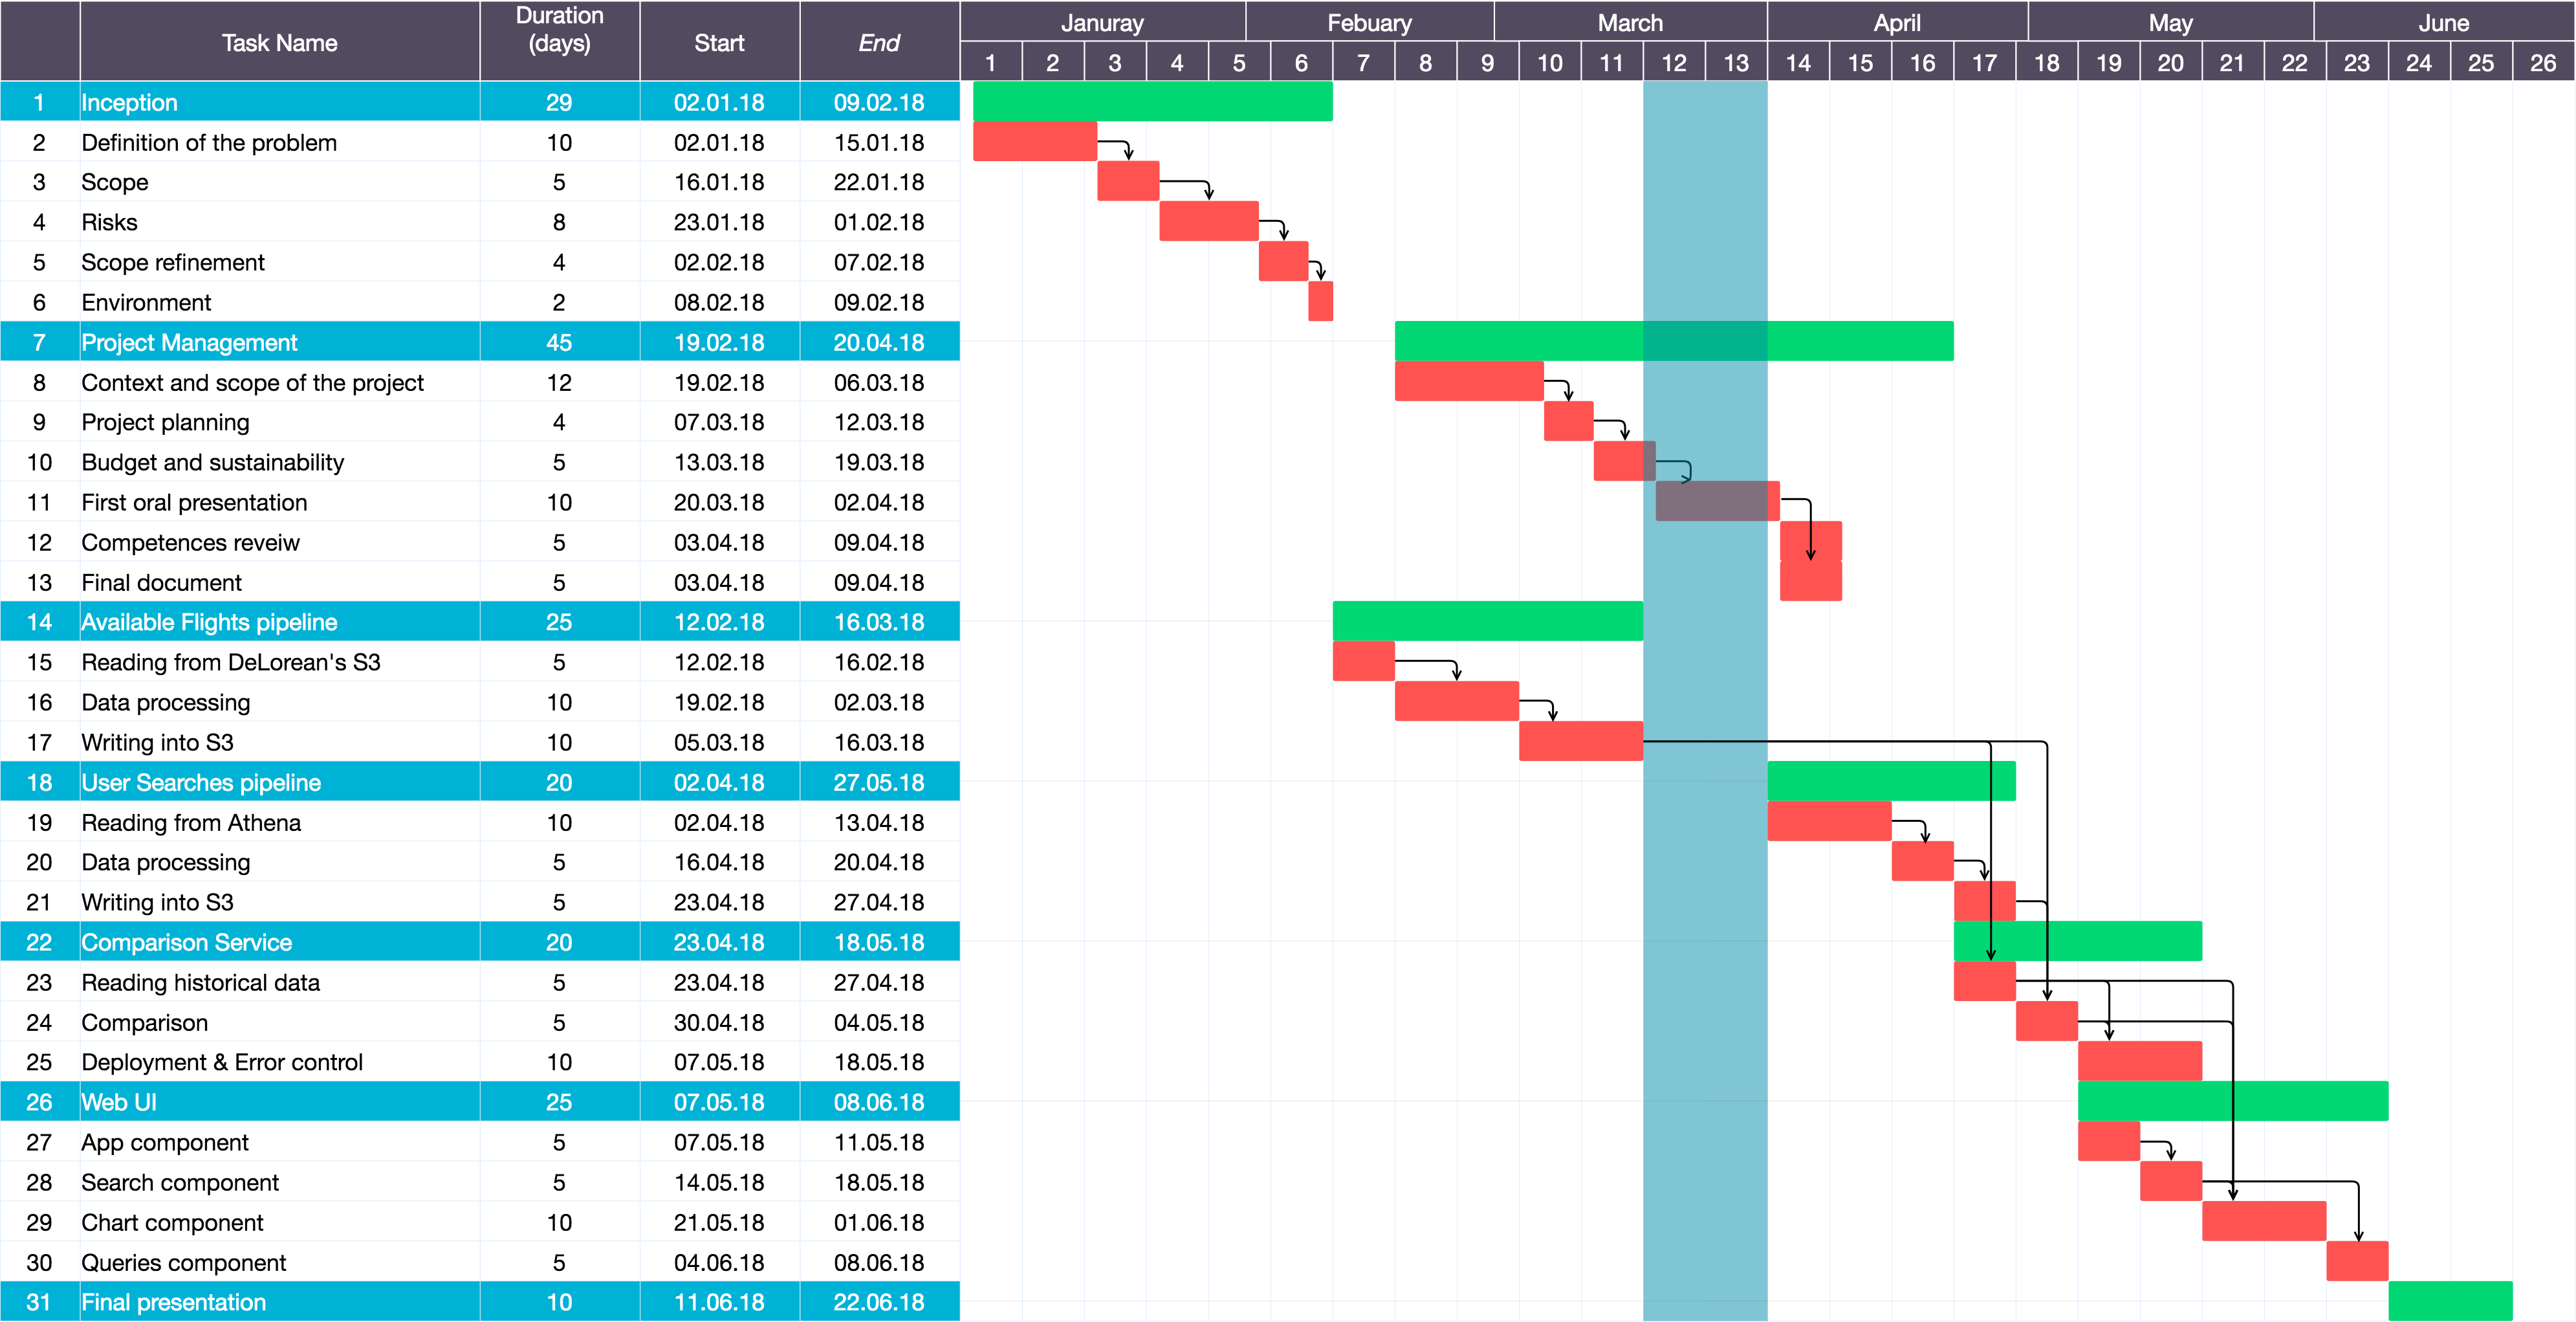
\includegraphics[scale=0.175,  angle =90]{diagrams/gantt.png}
\caption{Gantt diagram.}
\end{figure}




% Chapter 6: Budget and sustainability

\chapter{Budget and Sustainability}

\label{chapter06}

\section{Budget}

Once the project is planned in time and its technologies are drafted, we can calculate the project’s budget.
Skyscanner is not economically transparent, even for the employees. So, this whole calculation will be approximated.
\\\\
First of all, we have to take into account the employees, which is only one and in Intern position, and also count the taxes.
\\\\
Apart from that, all the hardware material and software licenses. AWS costs will continue but since it is going to be used during the development for testing it is counted in the total budget.

\begin{table}[H]
\centering
\begin{tabular}{|l|l|l|l|l|}
\hline
\textbf{Concept}           & \textbf{Price per unit} & \textbf{Units} & \textbf{Amortization} & \textbf{Total £}   \\ \hline
\textbf{Salary}            & 28 (taxes included)     & 575 h          &                       & 16100              \\ \hline
\textbf{MacBook Pro}       & 1700                    & 1              & life cycle 8 years    & 210                \\ \hline
\textbf{JetBrains License} & 230                     & 1              & 1 year per developer  & 130                \\ \hline
\textbf{AWS S3}            & 0.023                   & 50 TB          &                       & 1150               \\ \hline
\textbf{AWS}               & EC2                     & 575 h          &                       & 213.325            \\ \hline
\textbf{Screen}            & 200                     & 2              & life cycle 4 years    & 100                \\ \hline
\textbf{Office}            & Uknown                  & 1              &                       & Uknown             \\ \hline
\textbf{TOTAL}             &                         &                &                       & \textbf{17903.325} \\ \hline
\end{tabular}
\caption{Budget calculation}
\label{budget-calculation}
\end{table}

\section{Sustainability}

\subsection{Economical}

In economic terms, this project is initially unsustainable. It uses resources from Skyscanner for a comparison that might be useful in the future for other projects, improving some services or advertisement.
\\\\
But, if this product is sell to providers, Skyscanner can take a lot of profit from them. It is a very valuable application for providers, since they could compare airlines offer with actual user demand. Letting them improve their flights distribution and make more money.

\subsection{Social}

The \thesistitle is not directly involving society, but, as explained before, if providers have access to the comparison, flights will improve in terms of traveler experience. Travelers will have accurate routes depending on what they really want.
\\\\
For example, imagine that X carrier have several flights from BCN to ORY, Paris, and a few from BCN to FCO, Rome. The \thesistitle shows that the demand, compared with the offer is bigger in Rome than in Paris. Then, X airline could schedule more flights to FCO instead of ORY.

\subsection{Environment}

The environmental impact of the \thesistitle is directly related with the social impact.
\\\\
Right now, some airlines may have half full flights. This means that the airplane is not taking its most advantage of the fuel. It could be carrying more people.
\\\\
If carriers know where flights are really needed those flight will be full of people, which means that the fuel a flight uses is profited at its most.
\\\\
Otherwise, if an offer is under requested, the flight is not giving all the profit it could.
In other words, fuel per person will decrease.

\subsection{Sustainability matrix}

In order to understand the general impact of the project, the following general rating and evaluation is provided:
\\\\
The economical impact will be rated in 7/10. It could be a 10/10 it is sell to providers. Air companies could pay a lot of money for the \thesistitle because of the information it provides.
\\\\
The social impact will get a 4/10. It does nothing good nor bad to the society, only if the application is sell to providers and they use it properly, it could make some good to the people. In the other hand, the software will not be free, it will be property of \company.
\\\\
The environmental impact is a 4/10 as well. The environmental impact could be good if the application is sell to providers and they use it properly, but for now will not be sell to anyone. It gets a 4 because it will be using Amazon Web Service, and those machines are powered mainly by non-renewable energy\cite{click_clean}.
\\\\

\begin{table}[H]
\centering
\begin{tabular}{|l|l|l|}
\hline
Economical & Social & Environmental \\ \hline
7/10       & 4/10   & 4/10          \\ \hline
\multicolumn{3}{|l|}{15/30}         \\ \hline
\end{tabular}
\caption{Sustainability matrix}
\label{sustainability-matrix}
\end{table}



%----------------------------------------------------------------------------------------

%----------------------------------------------------------------------------------------
%	THESIS CONTENT - APPENDICES
%----------------------------------------------------------------------------------------

\appendix % Cue to tell LaTeX that the following "chapters" are Appendices

% Include the appendices of the thesis as separate files from the Appendices folder
% Uncomment the lines as you write the Appendices

\chapter{\company\ structure} 

\label{appendix_a}

\company\ has a very horizontal structure, based on Spotify's\cite{culture_of_growth}.
\\\\
In the top of the company hierarchy there is Gareth Williams (CEO and Co-founder). Bellow the rest of CxOs: CCO, CTO, CPO, CFO, CLO and the Senior Executive Assistant. Then vice presidents, senior managers, managers and then developers and interns\cite{crew_chart}.
\\\\
Apart from this hierarchy structure, the whole team, except the CEO, CxOs and the Senior Executive Assistant, is mainly split in \textbf{Squads}, each of those belong to a \textbf{Tribes}. Apart from Squads and Tribes there are also Chapters, Guilds ans XBT'S\cite{how_skyscanner_works}.

\section{Squad}

Are independent teams of no more than 8 people that are focused on delivering a core mission. Each squad has the freedom to act and be accountable to its mission.

\section{Tribe}

Squads belong to a Tribe. The tribe will have an aligning mission linking to each squad's mission and is only achievable depending on the success of each squad. The Tribe lead is responsible for providing the right environment to deliver and providing direction. 

\section{Chapters}

Are people who do similar work. This is a secondary home, and how people are line managed. Chapter leads are responsible for developing people and in tribe practices.

\section{Guilds}

Are communities of interest of people who do not necessarily do similar work. It is people from across the business that want to share knowledge, tools, and word practices. 

\section{XBT'S (cross business teams)}

XBTS' provide a platform to help solve business problems or opportunities with no natural home while giving all employees the ability to make an impact across any area of \company.

%----------------------------------------------------------------------------------------
%   BIBLIOGRAPHY
%----------------------------------------------------------------------------------------

\printbibliography[heading=bibintoc]

\end{document} 